\documentclass[times, 10pt,twocolumn]{article} 
\usepackage{mapnoreduce-report-g03}
\usepackage{times}
\usepackage{graphicx}
\usepackage[utf8x]{inputenc}
\usepackage{enumitem}
\usepackage{amsmath}
\usepackage{bm}
\usepackage{wasysym}
\usepackage{amsfonts}%
\usepackage{amssymb}%
\usepackage{graphicx}
\usepackage{fixltx2e}
\usepackage{color} 
\usepackage{colortbl}
\usepackage{subfig}
\usepackage{url}
\usepackage{cite}
\usepackage[portuguese, english]{babel} 
\usepackage{threeparttable}
\PassOptionsToPackage{hyphens}{url}\usepackage{hyperref}
\usepackage[hyphens]{url}\hypersetup{breaklinks=true}
\usepackage[square,sort,comma,numbers]{natbib}
\usepackage{tabularx}
\usepackage{booktabs}
\usepackage{chngpage}
\usepackage{pdflscape}
\usepackage[table]{xcolor}
\definecolor{lightgray}{gray}{0.9}
\usepackage{tikz}
\usepackage[printonlyused,nolist]{acronym}

\pagestyle{empty}

\begin{document}
	\title{MapNoReduce Platform}
	
	\author{
        João Pinho\\jpe.pinho@gmail.com\and Diogo Rosa\\
        diogo.m.c.rosa@gmail.com\and Cláudia Filipe\\
        claudia.p.b.filipe@gmail.com\\\\		 
		Instituto Superior Técnico\\
        Middleware for Distributed Internet Applications\\
        Lisbon, Portugal
    }
	\maketitle
	\thispagestyle{empty}
	
	\begin{abstract}
		This project consists in the design and implementation of MapNoReduce Platform, a simplified implementation of the MapReduce middleware and programming model. This platform extracts the input key/value pairs from input files and distributes the Map calls, called Jobs, across multiple machines, the Workers. 
		Also, the platform ensures a good performance by monitoring job's progress, detecting faulty or slow machines and rescheduling their tasks on idle machines. That is assured by Job Trackers, which are distributed in this platform, in contrast to the original implementation of MapReduce, where they are centralized. This mechanism was implemented inspired in Facebook's solution—Corona~\cite{ChingFacebook2012}. 
		Additionally, in order to test the platform it was developed a PuppetMaster component which allows to control the platform, and also to induce some delays and faults to the system in order to perform some tests and evaluation.
	\end{abstract}
    
	\section{Introduction}
	MapReduce was introduced by Google in 2004~\cite{GhemawatMR2008} and is currently one of the most popular approaches for large scale data analytics - also thanks to the availability of high quality open-source implementations. When using the MapReduce paradigm, the computation takes a set of input key/value pairs, and produces a set of output key/value pairs. MapReduce users express the computation as two functions: Map and Reduce. 
	This project focuses only the Map part, which uses a Map function given by the user and an input set of key/value pairs to produce a set of key/value pairs. 
	In MapNoReduce Platform the keys are the numbers of the line of the file being read and the values are the content of those lines.
    The Map invocations, called Jobs, are distributed across multiple machines by automatically partitioning the input data into a set of splits of size S. The input splits can be processed in parallel by those machines, named Workers. The system ensures that for each job submitted, all the input data is processed with a good performance through the monitoring of jobs' progress, fault or slow machines detection and reschedule of idle machine's tasks.
	In the original MapReduce implementation these tasks are performed by the JobTracker which is a centralized component. If the JobTracker fails the system can't receive new jobs nor processing pending ones, which can be critical in systems that need high availability.
	Considering JobTracker as a single point of failure~\cite{Kalavri2013}, it is necessary to replicate this component. As it would add complexity to the system and overhead, this project also introduces a new entity, the CoordinationManager, separating cluster resource management from job coordination, which allows the system to focus on make faster scheduling tasks.  
	
	\section{MapNoReduce Architecture}
		
        MapNoReduce is a simplified implementation of the MapReduce middleware and programming model, focused on the Map part. On this simplified version, our work provides a solution to common problems related with the reference architecture of the MapReduce platform. Those problems are related with fault-tolerance, replication and performance and will be discussed in the next sections. Additionally, we added some features that enable the overall testing of the system, such as the ability to run scripts over one or more functional servers or the capacity to monitor the system state while running those scripts.
        
        \begin{figure}[!h]
            \begin{center}
                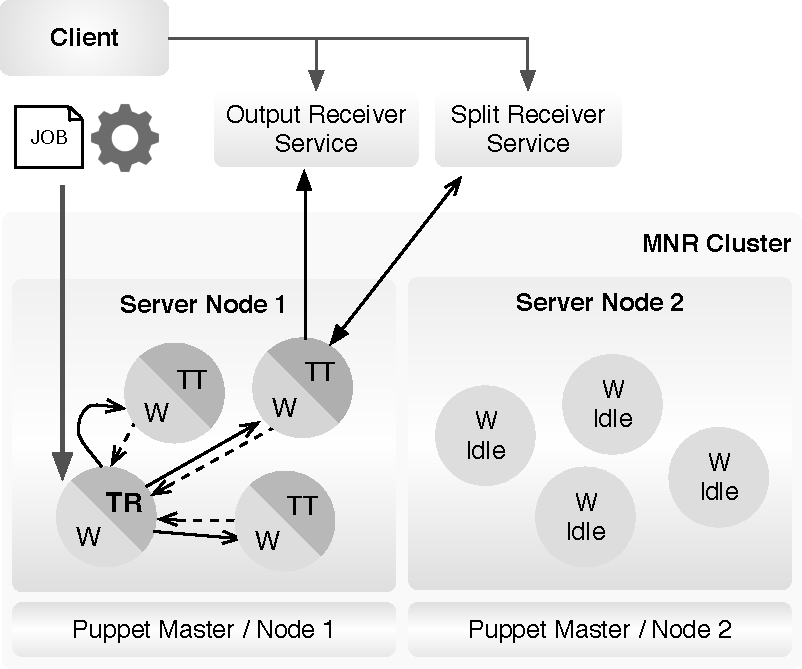
\includegraphics[width=0.48\textwidth]{pics/architecture.pdf}
                \caption{We illustrate an example of the MapNoReduce architecture. We represent one cluster with two server nodes. Inside the processing node, one JobTracker coordinates with other TaskTrackers to process the client job.  }
                \label{fig:mnr-architecture}
            \end{center}
        \end{figure}
        
    	\subsection{Worker}
    
    	\subsection{Job Tracker}
    	
        \subsubsection{Task Runner}

        \subsubsection{Task Tracker}

    	\subsubsection{Job Scheduler}
        
        \subsection{Replication}
        
        	\subsubsection{Coordination Manager}
        	
        	\subsubsection{Slave Replica}
    	
    	\subsection{Cluster Resource Management}
    	
            \subsubsection{Fair Share Scheduler}
        
    	\subsection{Puppet Master}
        
            \subsubsection{Management Interface}
            
            \subsubsection{Create Worker}
            
            \subsubsection{Status}
                	
            \subsubsection{Wait}
            
            \subsubsection{Slow Worker}
            
            \subsubsection{Freeze/Unfreeze Worker}
            
            \subsubsection{Freeze/Unfreeze Communication}
	
	\section{Evaluation}
	
	\section{Conclusions}
	
	\bibliographystyle{mapnoreduce-report-g03}
	\bibliography{mapnoreduce-rpt-g03}
\end{document}